
\section{Etapas del proyecto}
\label{sec:etapas}
En la figura \ref{fig:fig4} se muestran las distintas etapas del proyecto a realizar, diferenciando claramente las mismas y las tareas que componen a cada una de ellas.
\begin{figure}[ht]
  \centering
  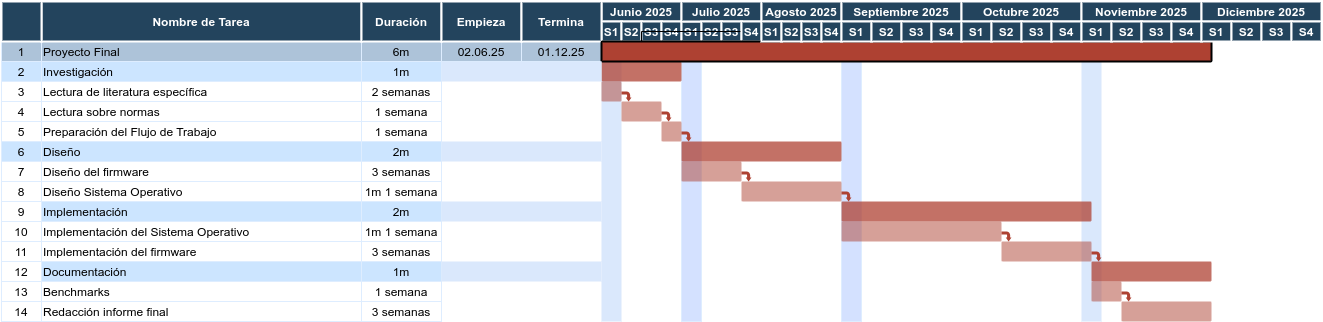
\includegraphics[width=1\textwidth]{figures/4.png}
  \caption{\label{fig:fig4}Planificación del proyecto}
\end{figure}

\pagebreak
\newpage

\begin{enumerate}
\item Se da inicio al proyecto.
\item La etapa de investigación consistirá de la búsqueda y lectura de la literatura especifica del tema, como lo es \cite{De_Vleeschauwer_2017}, con el fin principalmente de poder definir claramente las especificaciones del proyecto.
\item Luego se procede a la lectura y comprensión de la norma vigente para MPEG-2 (ISO/IEC) como se detalla en la bibliografía.
\item Finalmente en esta etapa de investigación incluimos la preparación del flujo de trabajo descrito en la Sección \ref{sec:metodologia}.
\item Pasando ya a la etapa de diseño corresponde comenzar con el dimensionamiento y la arquitectura del firmware, es decir proceder con la maqueta de las tareas de control y monitoreo, y estructura del archivo de registros de configuración, así como la definición de las interfaces y de la estructura en si de la API.
\item Una vez definido el firmware, resulta mas fácil delimitar el tamaño y funcionalidades del sistema operativo, que a priori por tratarse de un sistema en hardware, se tratará de un sistema operativo en tiempo real. Resulta conveniente realizarlo de esta manera para así no cometer errores de sobre diseño para con el sistema operativo.
\item Pasamos a la etapa de implementación, donde ahora se invierte la lógica pues resulta impráctico implementar el firmware sin un sistema operativo que servirá de plataforma cuando vayamos al chip en la vida real. Aquí entonces se realiza una implementación del sistema operativo en tiempo real para un subsistema de 4 microprocesadores RISC-V.
\item Ahora si procedemos con la implementación de las tareas propias del firmware con sus respectiva documentación técnica.
\item Pasamos a la etapa final de documentación. En primer lugar se ejecutarán distintos benchmarks para poder contrastar no solo la performance de nuestro sistema sino también de cada componente, es decir compararemos nuestro sistema operativo con otros comerciales o de amplia difusión, con un propósito más general.
\item Finalmente se dedicarán 3 semanas a la redacción del informe final que ha de ser presentado para la presentación del Proyecto Final.
\end{enumerate}
%%% Local Variables:
%%% mode: LaTeX
%%% TeX-master: "../anteproyecto"
%%% End:
